\documentclass[12pt]{article}

\usepackage{multicol}
\usepackage{textcomp}
\usepackage{amsmath,amssymb,amsfonts,latexsym,stmaryrd,graphicx}
\usepackage[utf8]{inputenc}
\usepackage[T1]{fontenc}
\usepackage{xcolor}
\usepackage{anyfontsize}
\usepackage[spanish]{babel}
\usepackage{listings}
\usepackage{latexsym}
\usepackage[pdftex,breaklinks,colorlinks,linkcolor=black,citecolor=black,urlcolor=black]{hyperref}

\usepackage{epstopdf}
\DeclareGraphicsExtensions{.pdf,.png,.jpg,.gif,.eps}

\newcommand{\proof}{\textbf{Demostración:} }
\newcommand{\nl}{\vspace{0.3cm}}

\newtheorem{theorem}{Teorema}
\newtheorem{lemma}{Lema}
\newtheorem{definition}{Definición}
\newtheorem{corollary}{Corolario}

%opening
\title{Proyecto de Diseño y Análisis de Algoritmos\\ \vspace{.2cm} \textbf{Finales Mundiales}}
\author{Leynier Gutiérrez González}

\begin{document}
	
\maketitle

\vspace{0.5cm}

\begin{center}
	\vspace{0.2cm}
	
\includegraphics[width=2.5cm]{images/escudo.png}\\
	\vspace{0.2cm}
	Facultad de Matemática y Computación\\
	\vspace{0.1cm}
	Universidad de La Habana\\
	\vspace{1cm}
\end{center}

\vspace{1cm}

\begin{abstract}
	En este documento se analizaran dos problemas de finales mundiales de la ACM International Collegiate Programming Contest.
\end{abstract}

\newpage

\tableofcontents

\newpage

\section{B - Comma Sprinkler - 2018}

\subsection{Descripción}

Como le dirá la práctica, las reglas en español para la colocación de comas son complejas, frustrantes y, a menudo, ambiguas. Mucha gente, incluso el inglés, en la práctica, los ignorará y aplicará reglas personalizadas, o, sin reglas, en absoluto. El Doctor Comma Sprinkler resolvió este problema desarrollando un conjunto de reglas que esparcen comas en una oración sin ambigüedad y poca simplicidad. En este problema, ayudará a la Dra. Sprinkler al producir un algoritmo para aplicar automáticamente sus reglas.

\nl

Las reglas del Dr. Sprinkler para agregar comas a un fragmento de texto existente son las siguientes:

\nl

Si una palabra en cualquier parte del texto va precedida por una coma, busque todas las apariciones de esa palabra en el texto y coloque una coma antes de cada una de esas ocurrencias, excepto en el caso de que tal ocurrencia sea la primera palabra de una oración o ya precedido por una coma.

\nl

Si una palabra en cualquier parte del texto es seguida por una coma, busque todas las apariciones de esa palabra en el texto y ponga una coma después de cada una de esas ocurrencias, excepto en el caso de que tal ocurrencia sea la última palabra de una oración o ya sucedido por una coma.

\nl

Aplique las reglas 1 y 2 repetidamente hasta que no se puedan agregar comas nuevas usando ninguna de ellas.

\nl

Como ejemplo, consideremos el texto.

\nl

\begin{tabular}{|c|}
	\hline please sit spot. sit spot, sit. spot here now here \\ 
	\hline 
\end{tabular} 

\nl

Debido a que hay una coma después de “spot” en la segunda oración, también debe agregarse una coma después de “spot” en la tercera oración (pero no la primera oración, ya que es la última palabra de esa oración). Además, debido a que hay una coma antes de la palabra “sit” en la segunda oración, se debe agregar una antes de esa palabra en la primera oración (pero no se agrega una coma antes de la palabra sentarse que comienza con la segunda oración porque es la primera palabra de esa oración). Finalmente, observe que una vez que se agrega una coma después de “spot” en la tercera oración, existe una coma antes de la primera aparición de la palabra “here”. Por lo tanto, también se agrega una coma antes de la otra aparición de la palabra “here”. No hay más comas que agregar, por lo que el resultado final es

\nl

\begin{tabular}{|c|}
	\hline please, sit spot. sit spot, sit. spot, here now, here. \\ 
	\hline 
\end{tabular} 

\subsubsection{Entrada}

La entrada contiene una línea de texto, que contiene al menos $2$ caracteres y como máximo $1000000$ caracteres. Cada carácter es una letra minúscula, una coma, un punto o un espacio. Definimos una palabra como una secuencia máxima de letras dentro del texto. El texto se adhiere a las siguientes restricciones:

\begin{itemize}
	\item El texto comienza con una palabra.
	\item Entre cada dos palabras en el texto, hay un espacio simple, una coma seguida de un espacio o un punto seguido de un espacio (que denota el final de una oración y el comienzo de una nueva).
	\item La última palabra del texto va seguida de un punto sin espacio al final.
\end{itemize}

\subsubsection{Salida}

Muestra el resultado después de aplicar el algoritmo de Dr. Sprinkler al texto original.

\begin{center}

	\nl
	
	\begin{tabular}{|c|c|}
		\hline Ejemplo de Entrada 1\\ 
		\hline please sit spot. sit spot, sit. spot here now here.\\
		\hline 
	\end{tabular} 
	
	\nl
	
	\begin{tabular}{|c|c|}
		\hline Ejemplo de Salida 1\\ 
		\hline please, sit spot. sit spot, sit. spot, here now, here.\\ 
		\hline 
	\end{tabular} 

\end{center}

\begin{center}
	
	\nl
	
	\begin{tabular}{|c|c|}
		\hline Ejemplo de Entrada 2\\ 
		\hline one, two. one tree. four tree. four four. five four. six five.\\
		\hline 
	\end{tabular} 
	
	\nl
	
	\begin{tabular}{|c|c|}
		\hline Ejemplo de Salida 2\\ 
		\hline one, two. one, tree. four, tree. four, four. five, four. six five.\\ 
		\hline 
	\end{tabular} 
	
\end{center}

\subsection{Solución}

La observación que se debe hacer aquí es que el problema se puede convertir en un problema de grafo. Crearemos dos vértices para cada palabra distinta en la entrada, uno que representa el comienzo de esa palabra y otro que representa el final. Conectamos el principio de la palabra $b$ con el final de la palabra $a$ si $a$ sigue inmediatamente a $b$ en cualquier oración del texto, lo que implica que si obtenemos una coma antes de $b$ en cualquier lugar del texto, también la colocaremos entre $a$ y $b$, y esto significa que pondremos una coma después de una $a$ en todas partes del texto (y viceversa).

\nl

Esto significa que si en la entrada original hay una coma después de alguna palabra $a$, y hay un camino desde $(a, fin)$ a $(c, fin)$ en la gráfica para algunos $c$, entonces también pondremos una coma después de cada aparición de $c$ en el texto y aplicaremos las reglas hasta que sea suficiente Por lo tanto, el problema es encontrar las componentes conexas en este grafo. Esto es factible con una aplicación de cualquier algoritmo de recorrido de grafos.

\nl

Así, comenzamos repasando el texto y construyendo el grafo. Podemos almacenar las palabras en una estructura de diccionario (como un mapa de C++), y para cada palabra en el texto, colocarla y actualizarla en el diccionario, si hay una coma después, marque eso en el diccionario, y si no está seguido de un punto, marcar la siguiente palabra como adyacente en el diccionario. En una sola pasada obtenemos suficiente información para construir el grafo. Ahora, colocamos los $(a, final)$ vértices en la cola de “visitar” y ejecutamos, digamos, el BFS, y finalmente reconstruimos el texto, poniendo una coma después de cada palabra no seguida por un período durante el cual $(a, final)$ ha sido visitada por la búsqueda.

\nl

Esto, se ejecutará, en el tiempo, $O(n\log(n))$, donde $n$, es el tamaño de la entrada que es lo suficientemente rápido.

\subsection{Código}

\href{https://gist.github.com/leynier/21d86c124811882b2474414f855f6bea}{gist.github.com/leynier/21d86c124811882b2474414f855f6bea}

\section{F - Go with the Flow - 2018}

\subsection{Descripción}

En la composición tipográfica, un “río” es una cadena de espacios formada por espacios entre palabras que se extiende hacia abajo varias líneas de texto. Por ejemplo, la figura de abajo muestra varios ejemplos de ríos resaltados en rojo (el texto es
intencionalmente borrosa para hacer los ríos más visibles).

\begin{center}
	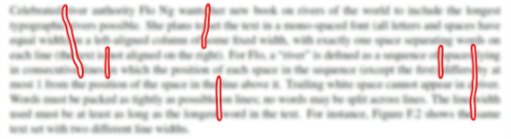
\includegraphics[width=10cm]{images/image1.png}
\end{center}

La célebre autoridad fluvial Flo Ng quiere que su nuevo libro sobre los ríos del mundo incluya los más largos ríos tipográficos posibles. Ella planea establecer el texto en una fuente mono-espaciada (todas las letras y espacios tienen ancho igual) en una columna alineada a la izquierda de un ancho fijo, con exactamente un espacio separando palabras en
Cada línea (el texto no está alineado a la derecha). Para Flo, un “río” se define como una secuencia de espacios que se encuentran en líneas consecutivas en las que la posición de cada espacio en la secuencia (excepto la primera) difiere en al más 1 de la posición del espacio en la línea por encima de él. El espacio en blanco que se arrastra no puede aparecer en un río. Las palabras deben estar empaquetadas lo más apretadamente posible en las líneas; no se pueden dividir palabras en líneas. El ancho de línea utilizado debe ser al menos tan largo como la palabra más larga en el texto. Por ejemplo, la figura de abajo muestra el mismo conjunto de texto con dos anchos de línea diferentes.

\begin{center}
	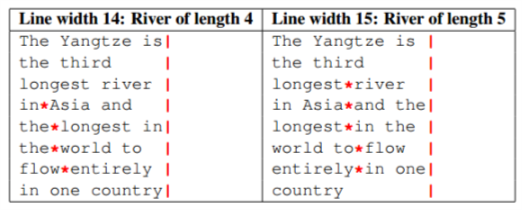
\includegraphics[width=8cm]{images/image2.png}
\end{center}

Dado un texto, se le ha asignado la tarea de determinar el ancho de línea que produce el río más largo de espacios para ese texto.

\subsubsection{Entrada}

La primera línea de entrada contiene un entero $n$ $(2 \leqslant n \leqslant 2500)$ que especifica el número de palabras en el texto. Las siguientes líneas de entrada contienen las palabras de texto. Cada palabra consta solo de letras minúsculas y mayúsculas, y las palabras en la misma línea están separadas por un solo espacio. Ninguna palabra supera los $80$ caracteres.

\subsubsection{Salida}

Muestra el ancho de línea para el cual el texto de entrada contiene el río más largo posible, seguido por la longitud del río más largo. Si más de un ancho de línea produce este máximo, muestre el ancho de línea más corto.

\begin{center}
	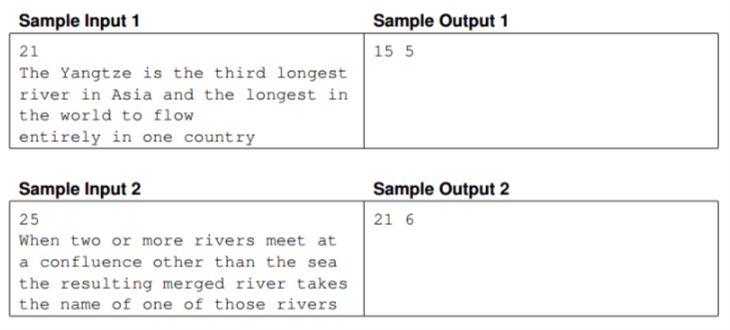
\includegraphics[width=13cm]{images/image3.png}
\end{center}

\subsection{Solución}

Para dar una solución a este problema, se puede probar que para todas las longitudes de líneas máximas, cual seria la que tuviese el rió de mayor longitud. Se podría realizar empezando desde la longitud mínima, o sea, la longitud de la palabra más larga del texto, y por cada palabra conocer si en el línea anterior existe un río y el tamaño de este; hasta que la longitud de la línea sea muy grande, de modo que todo el texto cupiese en una única línea y por tanto todos los ríos tuviesen longitud $1$. El límite del ejercicio en cuanto a tiempo es muy holgado, así que con una búsqueda optimizada o podándola se puede resolver el problema de una forma segura para el tiempo que se le ha otorgado. 

\nl

Ya que comenzaremos la búsqueda desde la mayor cantidad de líneas posibles, ya que se comienza por la menor longitud de líneas posibles, entonces se puede notar que el número de líneas va a decrecer a medida que esta simulación progrese, por tanto, si durante este proceso detectamos un río de longitud $L$, y llegamos al paso donde el número de líneas es $L$, entonces es obvio de que no encontraremos un río de longitud mayor que $L$. Esta sería nuestra optimización, detener la búsqueda cuando la cantidad de líneas actuales sea igual a la longitud del mayor río encontrado. De esta forma nos quitamos muchas iteraciones. En caso de la longitud del río sea un valor muy pequeño, de modo
de que teóricamente la búsqueda sea muy larga y la poda no tenga mucho efecto en la eficiencia del algoritmo, igual se necesitarían comprobar todas las longitudes de líneas anteriores para asegurar de que la longitud de río encontrada es la óptima. La complejidad temporal del algoritmo es $O(n^2*L^2)$ ya que existen a lo sumo $n*L$ longitudes de línea, donde $L$ es la longitud de la mayor palabra (en este caso acotado inferioremente por 80), y encontrar ríos en una línea de la forma propuesta es $O(n * L)$.

\subsection{Código}

\href{https://gist.github.com/leynier/fcf4145e14531d99a6882ea449f15a15}{gist.github.com/leynier/fcf4145e14531d99a6882ea449f15a15}

\newpage

\nocite{*}
\bibliographystyle{unsrt}
\bibliography{world_finals}

\end{document}
